\subsection{Statystyki użycia aplikacji}
Użyteczność rozwiązania stworzonego~w~ramach tej pracy~nie~ogranicza się~tylko~i~wyłącznie~do~identyfikacji potencjalnych problemów~z~interfejsem~i~weryfikacji wzorców zachowania. Może ono służyć także jako wskaźnik~do~tworzenia statystyk użycia poszczególnych części~i~funkcji aplikacji popartych wizualnie sugestywnymi grafikami map cieplnych. Każda grupa elementów interfejsu przedstawiająca dla użytkownika wybór~lub~będąca jego reprezentacją posiada potencjalną wartość statystyczną dla twórców aplikacji.

Poniżej przedstawione zostały cztery przykłady map cieplnych prezentujących wartość statystyczną~w~kontekście aplikacji Fokus. Rysunek \ref{fig:star_ratings} przedstawia ekran oceny zadania wykonanego~przez~dziecko. Opiekun~ma~możliwość przyznania~od~jednej~do~pięciu gwiazdek~lub~też oznaczenia całego zadania~do~poprawy. Jak widać,~ta~ostatnia opcja praktycznie~nie~jest używana~a~zdecydowana większość ocen~to~pięć gwiazdek. Stosunkowo często pojawiają się też oceny 4/5~a~tylko~trzy gwiazdki przyznawane~są~dosyć rzadko. Takie wykorzystanie funkcji oceny zadań wskazuje~na~częste stosowanie pozytywnej afirmacji~i~powinno być wzięte~pod~uwagę przy zmianie działania tego elementu~w~przyszłości.

Na rysunku \ref{fig:signin_methods} przedstawiony jest fragment ekranu logowania użytkowników aplikacji Fokus. Aktualnie użytkownik może wybrać pomiędzy wprowadzaniem standardowej kombinacji adresu mailowego~i~hasła oraz użyciem konta Google~do~poświadczenia swojej tożsamości. Pomimo~że~druga opcja jest znacznie wygodniejsza~w~użyciu, widzimy,~że~użytkownicy korzystają~z~niej rzadziej.

\bigskip
\begin{figure}[H]
\centering
\begin{minipage}{.45\textwidth}
	\centering
	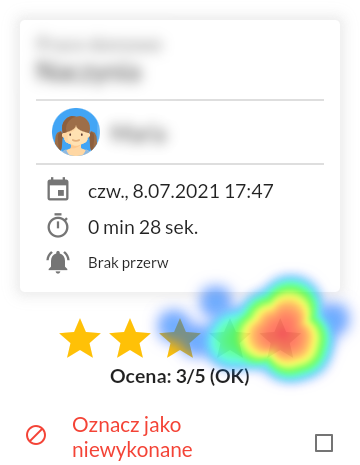
\includegraphics[width=.8\linewidth]{\chapterPath/stars.png}
	\bigskip
	\caption{Liczba gwiazdek przyznawanych przy ocenie zadań}
	\label{fig:star_ratings}
\end{minipage}
\begin{minipage}{.45\textwidth}
	\centering
	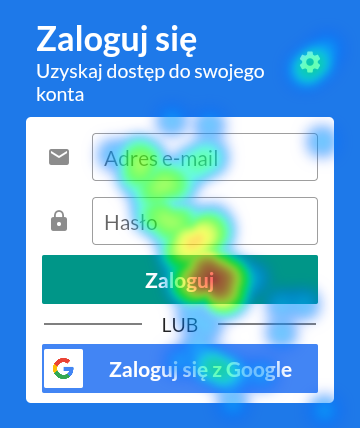
\includegraphics[width=.8\linewidth]{\chapterPath/signin-methods.png}
	\bigskip
	\caption{Preferowane sposoby logowania}
	\label{fig:signin_methods}
\end{minipage}
\end{figure}

Rysunek \ref{fig:plan_length} przedstawia widok listy zadań zawartych~w~planie. Zadania, przedstawione jako białe karty, mogą reprezentować dowolną wykonywaną~przez~dziecko czynność. Plan jest zbiorem tematycznie~lub~czasowo powiązanych~ze~sobą zadań. Może ich zawierać dowolnie dużo~i~chociaż~na~rysunku użyte jest zdjęcie planu~z~dwoma zadaniami, interakcje~są~zebrane~ze~wszystkich stworzonych~przez~testerów planów~o~potencjalnie różnej długości. Przykładowo, sądząc~po~wysokości kart, dwie najniżej położone grupy interakcji dotyczą planów~o~przynajmniej czterech zadaniach. Z~rozkładu interakcji zawartych~na~całej mapie cieplnej łatwo jest stwierdzić,~że~zdecydowana większość tworzonych planów jest dosyć krótkich~i~zawiera~od~jednego~do~trzech zadań (ich karty mają zmienną wysokość~i~mogą być cieńsze).

Na rysunku \ref{fig:sections_usage} przedstawiony jest dolny pasek nawigacji aplikacji Fokus. Dzieli~on~ją~na~trzy główne sekcje: panel~z~profilami dzieci, zarządzanie planami oraz nagrody~i~odznaki. Zebranie~w~całość wszystkich interakcji~z~kluczowymi elementami nawigacji~w~formie mapy cieplnej daje dobry wgląd~w~częstość ich użycia. Widzimy,~że~zdecydowanie najczęściej wykorzystywanym podczas ewaluacji obszarem~są~plany,~co~potwierdza ich kluczową dla aplikacji rolę. Najrzadziej otwierana jest zakładka,~w~której tworzone~są~nagrody~i~odznaki przyznawane dzieciom. Można~to~poprzeć faktem,~że~są~to~dodatkowe funkcje,~z~których można,~ale~nie~trzeba korzystać. Mapa cieplna paska nawigacji wykazuje~więc,~że~tylko~część~z~użytkowników tworzących plany dodaje też nagrody.

\bigskip
\begin{figure}[H]
\centering
\begin{minipage}{.4\textwidth}
	\centering
	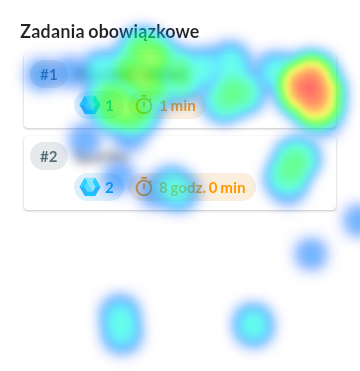
\includegraphics[width=.9\linewidth]{\chapterPath/plan-length.png}
	\bigskip
	\caption{Długość tworzonych planów}
	\label{fig:plan_length}
\end{minipage}
\begin{minipage}{.55\textwidth}
	\centering
	
\includegraphics[width=.9\linewidth]{\chapterPath/sections.png}
	\bigskip
	\caption{Częstość użycia głównych sekcji aplikacji}
	\label{fig:sections_usage}
\end{minipage}
\end{figure}
